\documentclass[leqno]{article}
\usepackage[utf8]{inputenc}
\usepackage{enumitem}
\usepackage{tikz}
\usepackage[parfill]{parskip}
\usepackage{mathtools}
\usepackage{amsmath}
\usepackage{amssymb}

\title{Computationele logica}
\author{
    Kamans, Jim\\
    \texttt{10302905}
    \and
    Roosingh, Sander\\
    \texttt{11983957}
    \and
    Schenk, Stefan\\
    \texttt{11881798}
}
\date{December 2017}

\begin{document}

\maketitle

\section*{Exercise 1}

\begin{enumerate}
	\item \textit{Represent the robot's belief-revision structure using a single-agent plausibility model,} with four possible states, using the atomic sentences $m$ for "there is a mine in front of the robot", and $e$ for "an enemy is approaching". Draw arrows going from the less plausible worlds to more plausible worlds (according to the robot's plausibility relation). In your drawing, you may skip the loops (since plausibility relations are assumed to be reflexive) and the arrows that can be obtained by composing other arrows (since plausibility relations are assumed to be transitive), but be aware that they are there. Also, be sure to use all information given in the text above.\\
	\begin{center}
		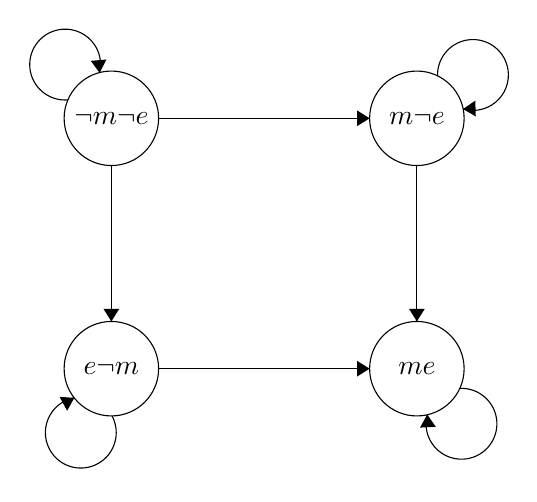
\begin{tikzpicture}[scale=0.2]
		\tikzstyle{every node}+=[inner sep=0pt]
		\draw [black] (46.3,-17) circle (3);
		\draw (46.3,-17) node {$m \neg e$};
		\draw [black] (26.9,-32.9) circle (3);
		\draw (26.9,-32.9) node {$e \neg m$};
		\draw [black] (26.9,-17) circle (3);
		\draw (26.9,-17) node {$\neg m \neg e$};
		\draw [black] (46.3,-32.9) circle (3);
		\draw (46.3,-32.9) node {$me$};
		\draw [black] (26.9,-20) -- (26.9,-29.9);
		\fill [black] (26.9,-29.9) -- (27.4,-29.1) -- (26.4,-29.1);
		\draw [black] (29.9,-32.9) -- (43.3,-32.9);
		\fill [black] (43.3,-32.9) -- (42.5,-32.4) -- (42.5,-33.4);
		\draw [black] (46.3,-20) -- (46.3,-29.9);
		\fill [black] (46.3,-29.9) -- (46.8,-29.1) -- (45.8,-29.1);
		\draw [black] (29.9,-17) -- (43.3,-17);
		\fill [black] (43.3,-17) -- (42.5,-16.5) -- (42.5,-17.5);
		\draw [black] (47.612,-14.315) arc (181.69424:-106.30576:2.25);
		\fill [black] (49.23,-16.41) -- (50.04,-16.88) -- (50.01,-15.88);
		\draw [black] (24.15,-15.831) arc (274.71268:-13.28732:2.25);
		\fill [black] (26.15,-14.11) -- (26.59,-13.27) -- (25.59,-13.35);
		\draw [black] (26.937,-35.888) arc (28.44003:-259.55997:2.25);
		\fill [black] (24.55,-34.75) -- (23.61,-34.69) -- (24.09,-35.57);
		\draw [black] (49.014,-34.151) arc (92.99099:-195.00901:2.25);
		\fill [black] (46.96,-35.81) -- (46.5,-36.64) -- (47.5,-36.59);
		\end{tikzpicture}
	\end{center}
	
	\item 
	\item 
	\item 
	\item 
	\item 
\end{enumerate}

\section*{Exercise 2}

\begin{enumerate}
	\item 
	\item 
	\item 
	\item 
	\item 
\end{enumerate}

\end{document}
